\section{Numerical Simulation}
\subsection{Detailed Simulation Results for Star Interaction Hamiltonian \texorpdfstring{\( H^{(1)} \)}{H1}}
\label{appendix:numerical-simulation}

In this appendix, we present a more comprehensive study of the teleportation protocols under the star-type Hamiltonian \( H^{(1)} \), focusing on the dependence of the results on the transverse field \( h \), while keeping the coupling strength \( J = 1 \) fixed.

\subsubsection{Teleportation Fidelity vs External Field \texorpdfstring{\( h \)}{h}}

The plots in Figure~\ref{fig:alice_vs_hJ} show the behavior of Bob's expectation values across varying values of \( h \) and \( J \) as completion to Figure~\ref{fig:alice_x_vs_j} from main text. We observe:

\begin{itemize}
    \item For \textbf{energy teleportation}, the fidelity degrades as \( h \) increases, due to the weakening of \( X_0 X_k \) correlations dominating the interaction term.
    \item For \textbf{charge teleportation}, a similar trend is observed, but the degradation is smoother, indicating better resilience to increasing transverse field strengths.
\end{itemize}

\begin{figure*}[t!]
    \centering
    \begin{subfigure}{0.24\textwidth}
        \centering
        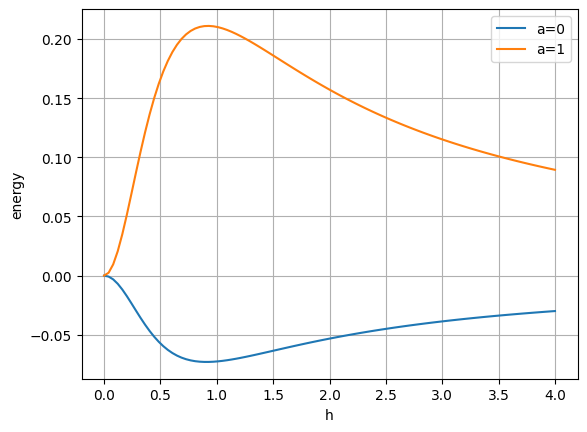
\includegraphics[width=\textwidth]{Appendix/plots/numerical/Alice/N1_energy_vs_h.png}
        \caption{Energy, \( N = 1 \), \( h \)}
    \end{subfigure}
    \hfill
    \begin{subfigure}{0.24\textwidth}
        \centering
        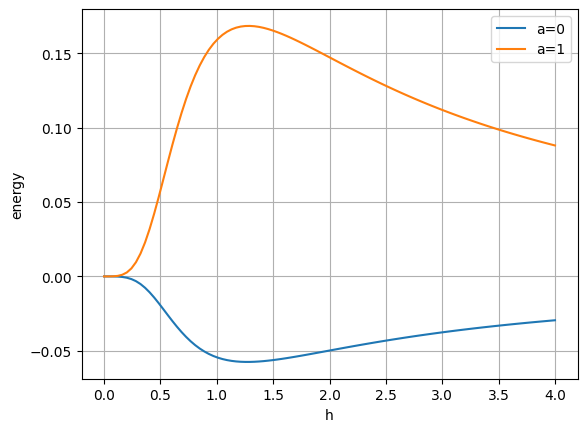
\includegraphics[width=\textwidth]{Appendix/plots/numerical/Alice/N2_energy_vs_h.png}
        \caption{Energy, \( N = 2 \), \( h \)}
    \end{subfigure}
    \hfill
    \begin{subfigure}{0.24\textwidth}
        \centering
        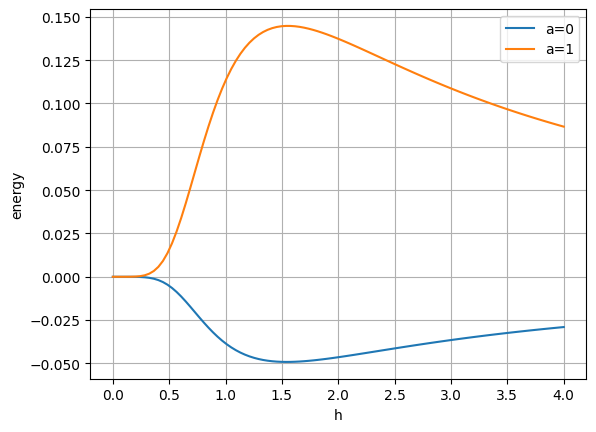
\includegraphics[width=\textwidth]{Appendix/plots/numerical/Alice/N3_energy_vs_h.png}
        \caption{Energy, \( N = 3 \), \( h \)}
    \end{subfigure}
    \hfill
    \begin{subfigure}{0.24\textwidth}
        \centering
        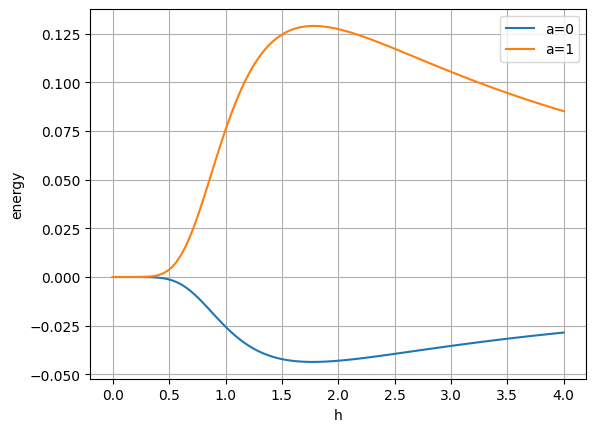
\includegraphics[width=\textwidth]{Appendix/plots/numerical/Alice/N4_energy_vs_h.png}
        \caption{Energy, \( N = 4 \), \( h \)}
    \end{subfigure}

    \vspace{0.5em}

    \begin{subfigure}{0.24\textwidth}
        \centering
        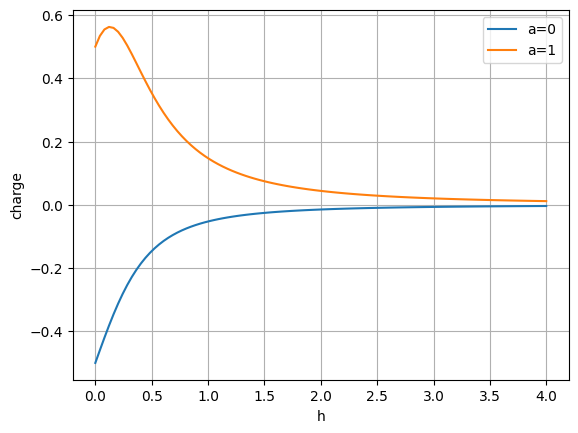
\includegraphics[width=\textwidth]{Appendix/plots/numerical/Alice/N1_charge_vs_h.png}
        \caption{Charge, \( N = 1 \), \( h \)}
    \end{subfigure}
    \hfill
    \begin{subfigure}{0.24\textwidth}
        \centering
        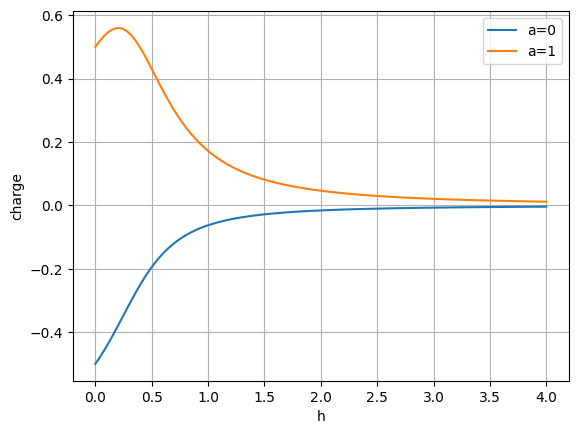
\includegraphics[width=\textwidth]{Appendix/plots/numerical/Alice/N2_charge_vs_h.png}
        \caption{Charge, \( N = 2 \), \( h \)}
    \end{subfigure}
    \hfill
    \begin{subfigure}{0.24\textwidth}
        \centering
        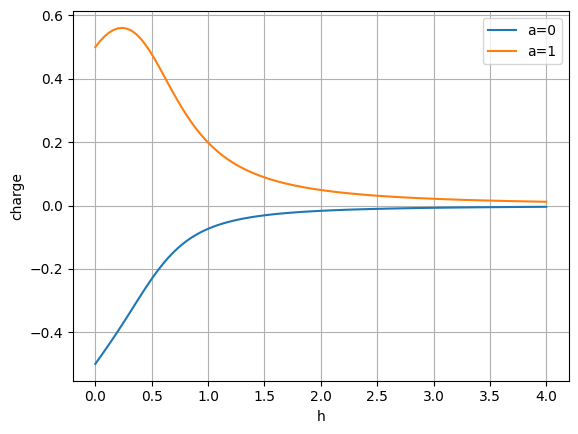
\includegraphics[width=\textwidth]{Appendix/plots/numerical/Alice/N3_charge_vs_h.png}
        \caption{Charge, \( N = 3 \), \( h \)}
    \end{subfigure}
    \hfill
    \begin{subfigure}{0.24\textwidth}
        \centering
        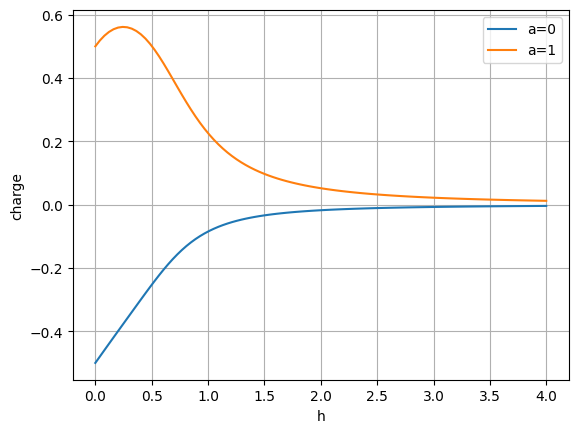
\includegraphics[width=\textwidth]{Appendix/plots/numerical/Alice/N4_charge_vs_h.png}
        \caption{Charge, \( N = 4 \), \( h \)}
    \end{subfigure}
    
    \vspace{0.5em}

    \begin{subfigure}{0.24\textwidth}
        \centering
        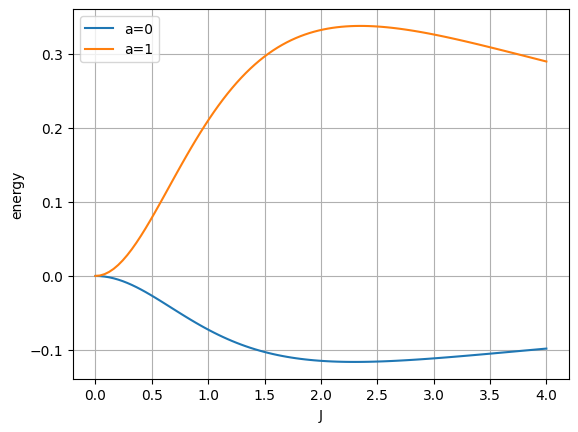
\includegraphics[width=\textwidth]{Appendix/plots/numerical/Alice/N1_energy_vs_J.png}
        \caption{Energy, \( N = 1 \), \( J \)}
    \end{subfigure}
    \hfill
    \begin{subfigure}{0.24\textwidth}
        \centering
        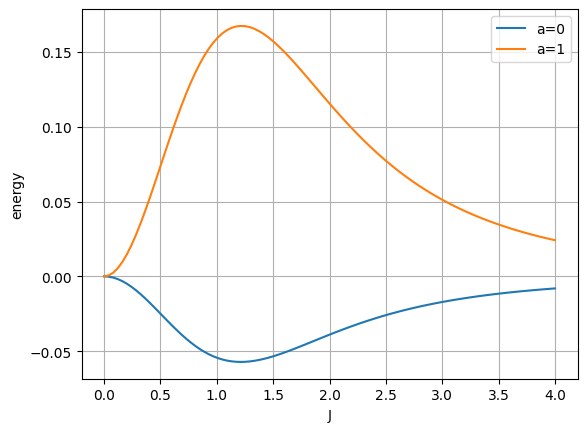
\includegraphics[width=\textwidth]{Appendix/plots/numerical/Alice/N2_energy_vs_J.png}
        \caption{Energy, \( N = 2 \), \( J \)}
    \end{subfigure}
    \hfill
    \begin{subfigure}{0.24\textwidth}
        \centering
        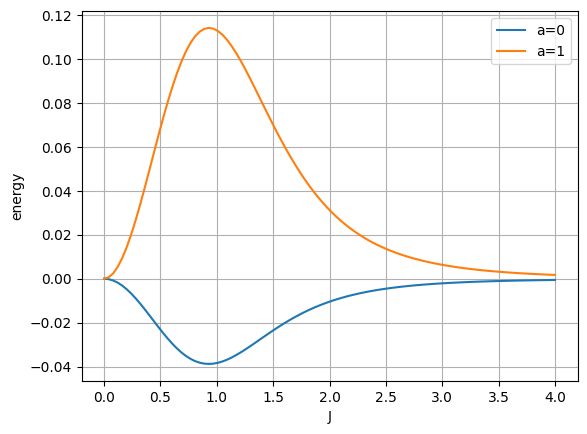
\includegraphics[width=\textwidth]{Appendix/plots/numerical/Alice/N3_energy_vs_J.png}
        \caption{Energy, \( N = 3 \), \( J \)}
    \end{subfigure}
    \hfill
    \begin{subfigure}{0.24\textwidth}
        \centering
        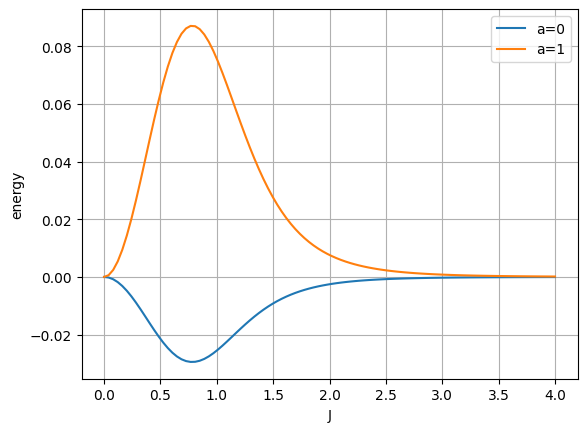
\includegraphics[width=\textwidth]{Appendix/plots/numerical/Alice/N4_energy_vs_J.png}
        \caption{Energy, \( N = 4 \), \( J \)}
    \end{subfigure}

    \caption{Extracted value at Bob's site, under Start-Interaction Hamiltonian for Energy and Charge.}
    \label{fig:alice_vs_hJ}
\end{figure*}

\subsubsection{Protocol Optimization and Design Implications}

From the simulations, we find that optimal teleportation occurs at intermediate field strengths and coupling ratios, typically where entanglement entropy is near its peak. This aligns with previous findings in~\cite{Ikeda2023, IkedaTeleportingCharge}. These results suggest:

\begin{itemize}
    \item Energy teleportation is more sensitive to parameter tuning, requiring careful Hamiltonian engineering.
    \item Charge teleportation, while delivering slightly smaller absolute observable values, is more stable and symmetric, offering better QKD performance under noise or imperfect conditions.
\end{itemize}

\subsubsection{Robustness to Bit Flipping}

As shown in both main text and simulations, the expectation values under charge teleportation exhibit perfect mirror symmetry under the bit-flipping of Alice’s result \( b \to b \oplus 1 \). This provides a useful check for correctness and a natural framework for encoding binary key bits, as emphasized in~\cite{QKDbyQET}.

These findings strengthen the case for preferring charge-based QKD implementations in practical systems, especially where channel errors or imperfect hardware may break energy teleportation asymmetries.

\subsection{Additional Results for Nearest-Neighbor Interaction}
\label{appendix:nn_detailed}

This appendix includes further numerical results for the nearest-neighbor Hamiltonian, focusing on the dependence of teleportation fidelity on the external field \( h \) for different measurement bases.

\subsubsection{Observable Expectation Values vs. \texorpdfstring{\( h \)}{h}}

Figures~\ref{fig:nn_vs_h_X},~\ref{fig:nn_vs_h_Y}, and~\ref{fig:nn_vs_h_both} present the behavior of teleported observables as a function of \( h \), with fixed coupling \( J=1 \). The trends are qualitatively similar to the \( J \)-dependence, but with more rapid decay in observable magnitude for large \( h \), due to the dominance of the local \( Z \)-field.

\begin{figure*}[t!]
    \centering
    \begin{subfigure}{0.33\textwidth}
        \centering
        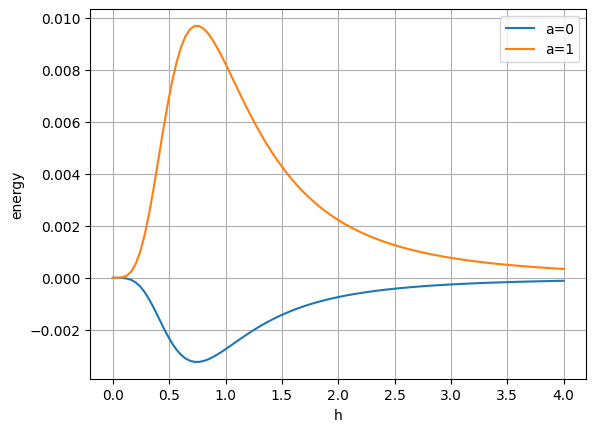
\includegraphics[width=\textwidth]{Appendix/plots/numerical/NearestNeighbors/X_N2_energy_vs_h.png}
        \caption{Energy, \( N = 2 \)}
    \end{subfigure}
    \hfill
    \begin{subfigure}{0.33\textwidth}
        \centering
        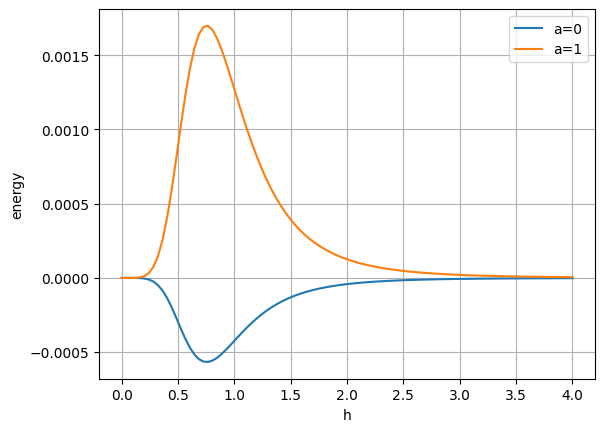
\includegraphics[width=\textwidth]{Appendix/plots/numerical/NearestNeighbors/X_N3_energy_vs_h.png}
        \caption{Energy, \( N = 3 \)}
    \end{subfigure}
    \hfill
    \begin{subfigure}{0.33\textwidth}
        \centering
        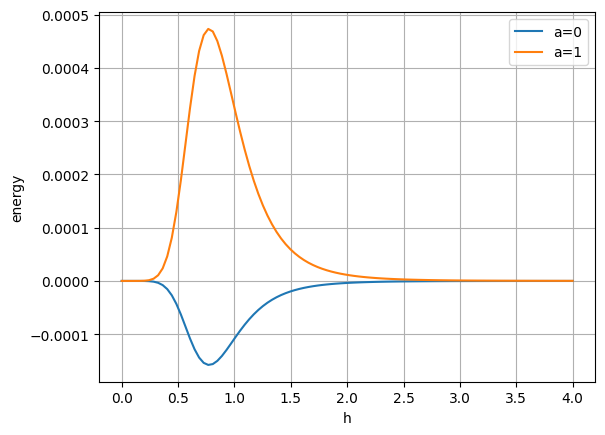
\includegraphics[width=\textwidth]{Appendix/plots/numerical/NearestNeighbors/X_N4_energy_vs_h.png}
        \caption{Energy, \( N = 4 \)}
    \end{subfigure}

    \vspace{0.5em}

    \begin{subfigure}{0.33\textwidth}
        \centering
        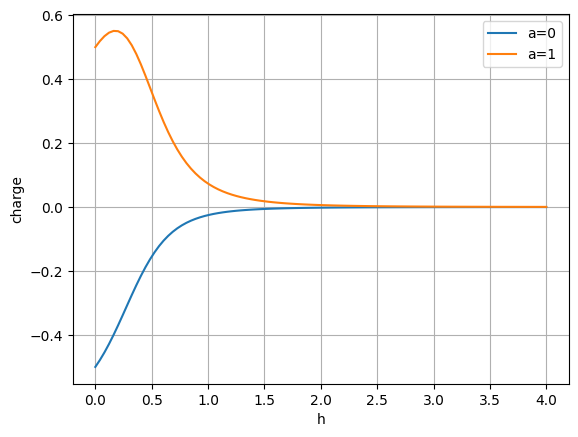
\includegraphics[width=\textwidth]{Appendix/plots/numerical/NearestNeighbors/X_N2_charge_vs_h.png}
        \caption{Charge, \( N = 2 \)}
    \end{subfigure}
    \hfill
    \begin{subfigure}{0.33\textwidth}
        \centering
        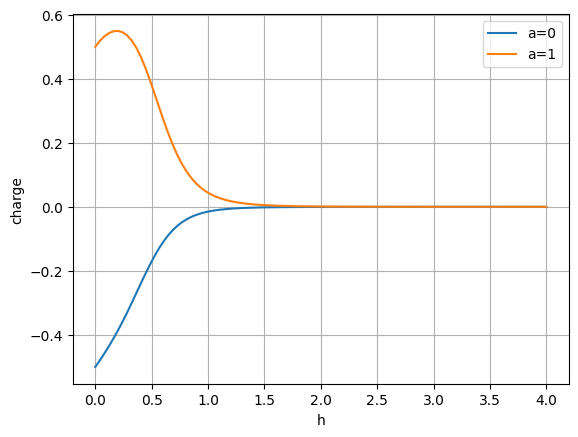
\includegraphics[width=\textwidth]{Appendix/plots/numerical/NearestNeighbors/X_N3_charge_vs_h.png}
        \caption{Charge, \( N = 3 \)}
    \end{subfigure}
    \hfill
    \begin{subfigure}{0.33\textwidth}
        \centering
        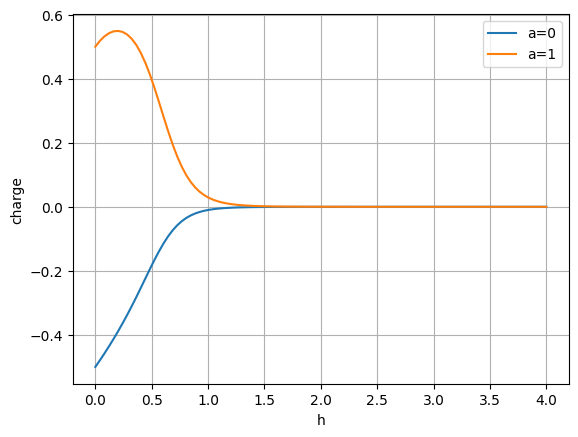
\includegraphics[width=\textwidth]{Appendix/plots/numerical/NearestNeighbors/X_N4_charge_vs_h.png}
        \caption{Charge, \( N = 4 \)}
    \end{subfigure}

    \caption{Extracted value at Bob's site vs. \( h \), under nearest-neighbor Hamiltonian for Energy and Charge for \( \sigma_A = X_0 \).}
    \label{fig:nn_vs_h_X}
\end{figure*}

\begin{figure*}[t!]
    \centering
    \begin{subfigure}{0.33\textwidth}
        \centering
        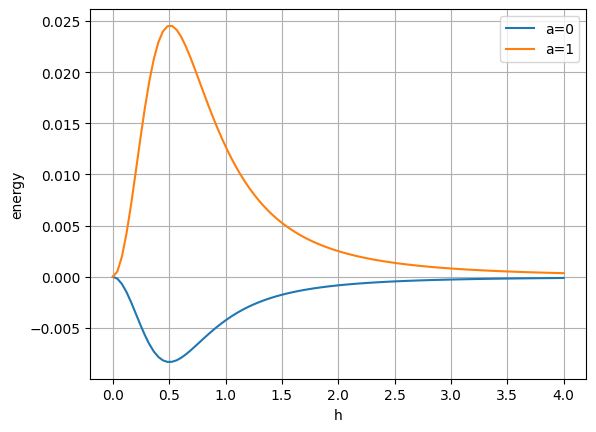
\includegraphics[width=\textwidth]{Appendix/plots/numerical/NearestNeighbors/Y_N2_energy_vs_h.png}
        \caption{Energy, \( N = 2 \)}
    \end{subfigure}
    \hfill
    \begin{subfigure}{0.33\textwidth}
        \centering
        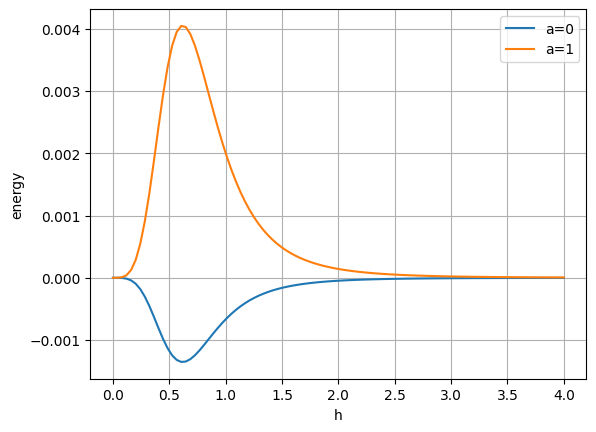
\includegraphics[width=\textwidth]{Appendix/plots/numerical/NearestNeighbors/Y_N3_energy_vs_h.png}
        \caption{Energy, \( N = 3 \)}
    \end{subfigure}
    \hfill
    \begin{subfigure}{0.33\textwidth}
        \centering
        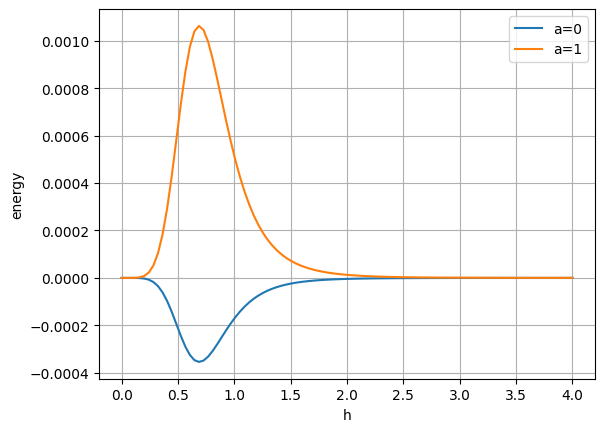
\includegraphics[width=\textwidth]{Appendix/plots/numerical/NearestNeighbors/Y_N4_energy_vs_h.png}
        \caption{Energy, \( N = 4 \)}
    \end{subfigure}

    \vspace{0.5em}

    \begin{subfigure}{0.33\textwidth}
        \centering
        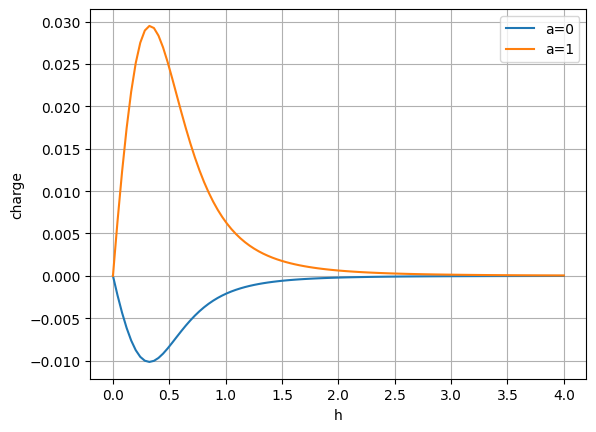
\includegraphics[width=\textwidth]{Appendix/plots/numerical/NearestNeighbors/Y_N2_charge_vs_h.png}
        \caption{Charge, \( N = 2 \)}
    \end{subfigure}
    \hfill
    \begin{subfigure}{0.33\textwidth}
        \centering
        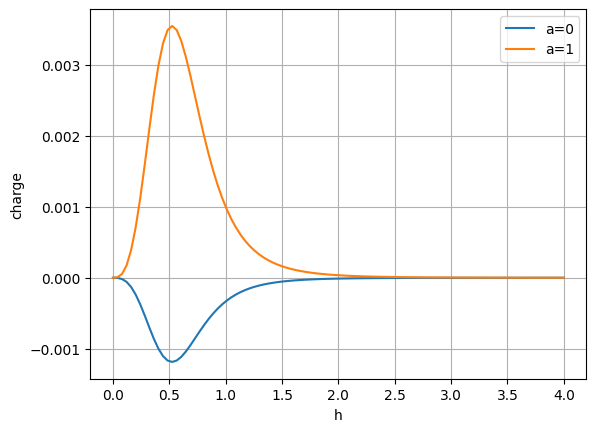
\includegraphics[width=\textwidth]{Appendix/plots/numerical/NearestNeighbors/Y_N3_charge_vs_h.png}
        \caption{Charge, \( N = 3 \)}
    \end{subfigure}
    \hfill
    \begin{subfigure}{0.33\textwidth}
        \centering
        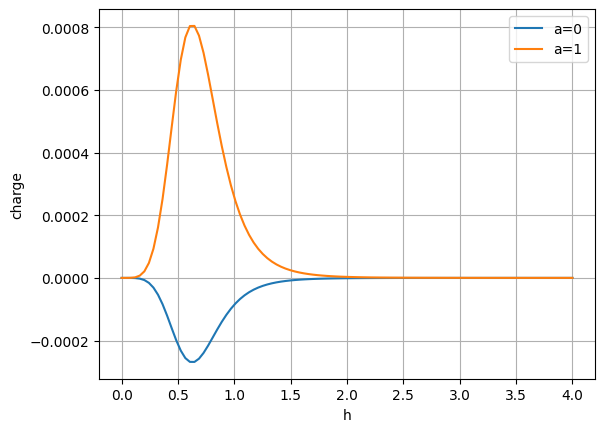
\includegraphics[width=\textwidth]{Appendix/plots/numerical/NearestNeighbors/Y_N4_charge_vs_h.png}
        \caption{Charge, \( N = 4 \)}
    \end{subfigure}
    
    \caption{Extracted value at Bob's site vs. \( h \), under nearest-neighbor Hamiltonian for Energy and Charge for \( \sigma_A = Y_0 \).}
    \label{fig:nn_vs_h_Y}
\end{figure*}
    
\begin{figure*}[t!]
    \centering
    \begin{subfigure}{0.33\textwidth}
        \centering
        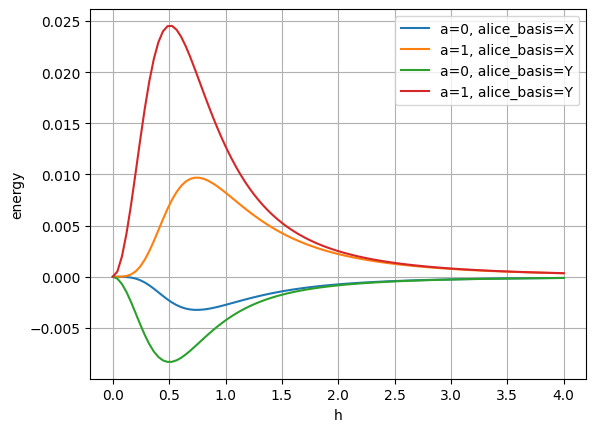
\includegraphics[width=\textwidth]{Appendix/plots/numerical/NearestNeighbors/both_N2_energy_vs_h.png}
        \caption{Energy, \( N = 2 \)}
    \end{subfigure}
    \hfill
    \begin{subfigure}{0.33\textwidth}
        \centering
        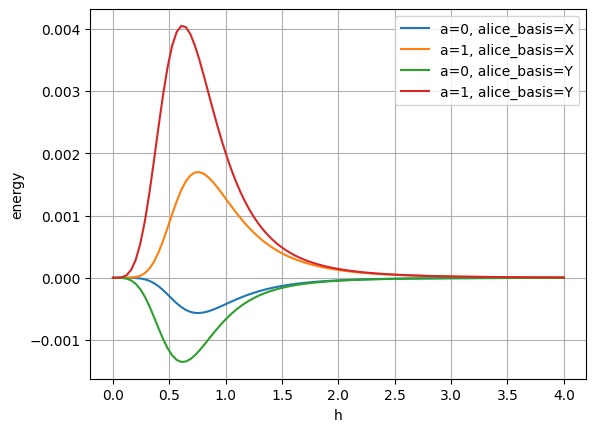
\includegraphics[width=\textwidth]{Appendix/plots/numerical/NearestNeighbors/both_N3_energy_vs_h.png}
        \caption{Energy, \( N = 3 \)}
    \end{subfigure}
    \hfill
    \begin{subfigure}{0.33\textwidth}
        \centering
        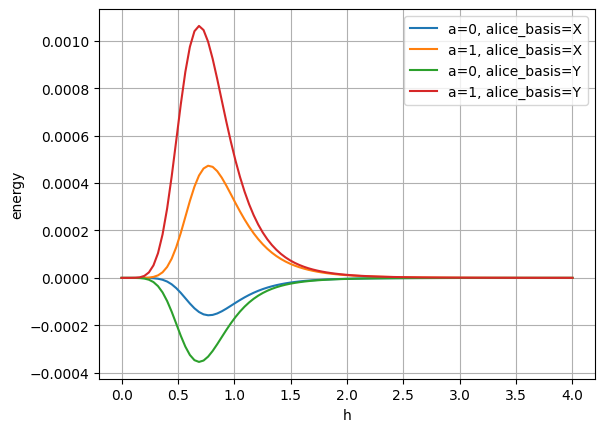
\includegraphics[width=\textwidth]{Appendix/plots/numerical/NearestNeighbors/both_N4_energy_vs_h.png}
        \caption{Energy, \( N = 4 \)}
    \end{subfigure}

    \vspace{0.5em}

    \begin{subfigure}{0.33\textwidth}
        \centering
        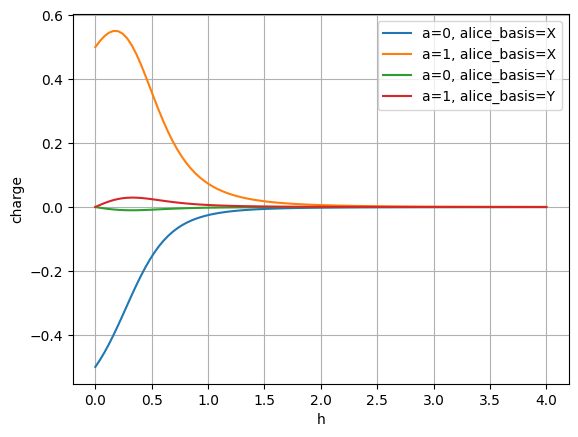
\includegraphics[width=\textwidth]{Appendix/plots/numerical/NearestNeighbors/both_N2_charge_vs_h.png}
        \caption{Charge, \( N = 2 \)}
    \end{subfigure}
    \hfill
    \begin{subfigure}{0.33\textwidth}
        \centering
        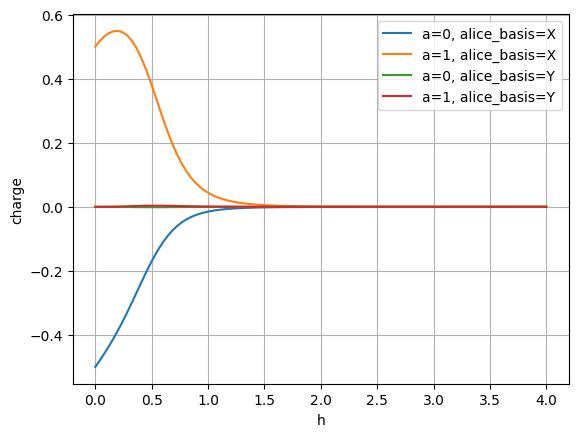
\includegraphics[width=\textwidth]{Appendix/plots/numerical/NearestNeighbors/both_N3_charge_vs_h.png}
        \caption{Charge, \( N = 3 \)}
    \end{subfigure}
    \hfill
    \begin{subfigure}{0.33\textwidth}
        \centering
        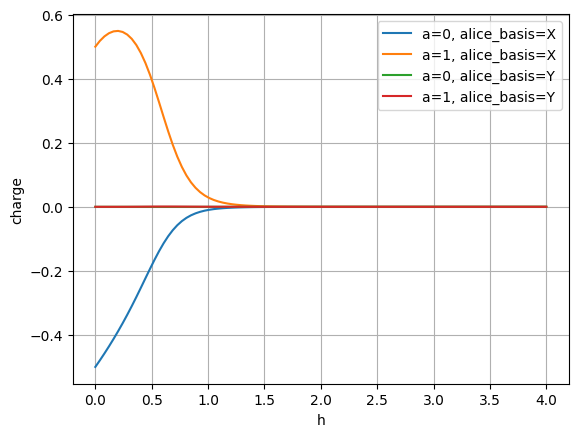
\includegraphics[width=\textwidth]{Appendix/plots/numerical/NearestNeighbors/both_N4_charge_vs_h.png}
        \caption{Charge, \( N = 4 \)}
    \end{subfigure}
    
    \caption{Extracted value at Bob's site vs. \( h \), under nearest-neighbor Hamiltonian for Energy and Charge for both Alice Bases.}
    \label{fig:nn_vs_h_both}
\end{figure*}

\begin{figure*}[t!]
    \centering
    \begin{subfigure}{0.33\textwidth}
        \centering
        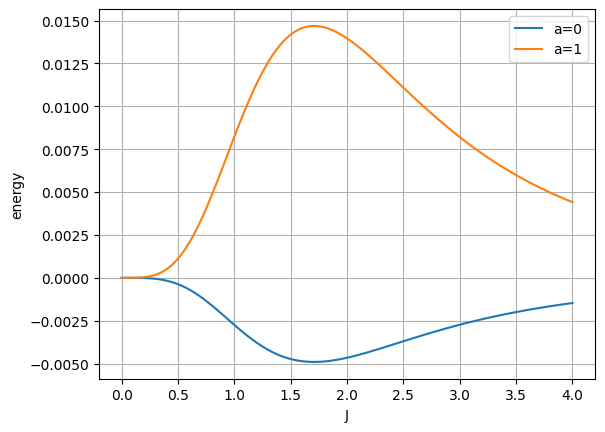
\includegraphics[width=\textwidth]{Appendix/plots/numerical/NearestNeighbors/X_N2_energy_vs_J.png}
        \caption{\( \sigma_A = X_0 \), \( N = 2 \)}
    \end{subfigure}
    \hfill
    \begin{subfigure}{0.33\textwidth}
        \centering
        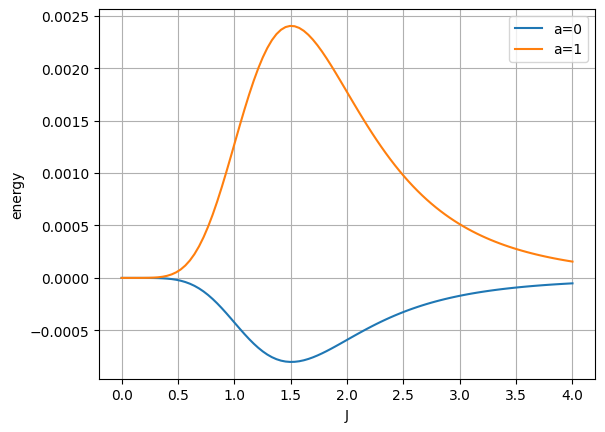
\includegraphics[width=\textwidth]{Appendix/plots/numerical/NearestNeighbors/X_N3_energy_vs_J.png}
        \caption{\( \sigma_A = X_0 \), \( N = 3 \)}
    \end{subfigure}
    \hfill
    \begin{subfigure}{0.33\textwidth}
        \centering
        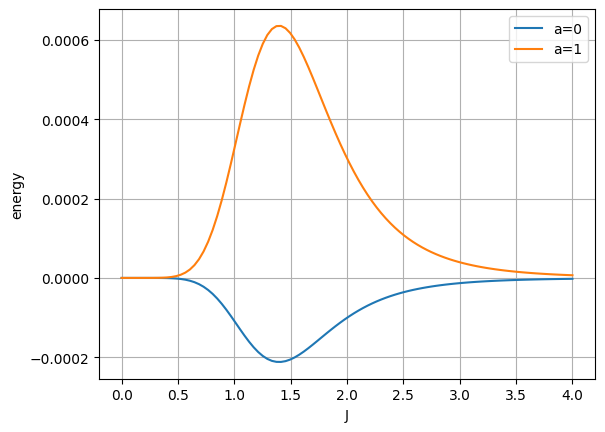
\includegraphics[width=\textwidth]{Appendix/plots/numerical/NearestNeighbors/X_N4_energy_vs_J.png}
        \caption{\( \sigma_A = X_0 \), \( N = 4 \)}
    \end{subfigure}

    \vspace{0.5em}

    \begin{subfigure}{0.33\textwidth}
        \centering
        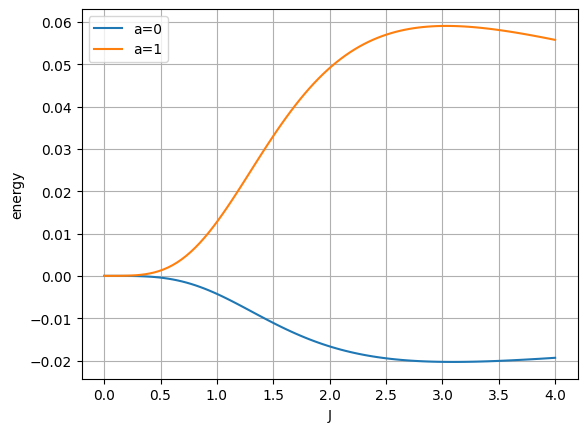
\includegraphics[width=\textwidth]{Appendix/plots/numerical/NearestNeighbors/Y_N2_energy_vs_J.png}
        \caption{\( \sigma_A = Y_0 \), \( N = 2 \)}
    \end{subfigure}
    \hfill
    \begin{subfigure}{0.33\textwidth}
        \centering
        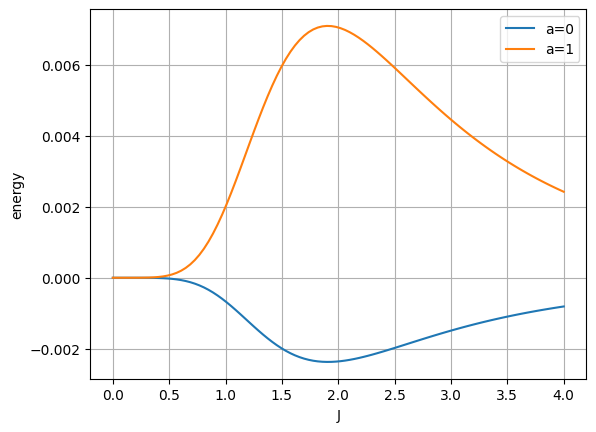
\includegraphics[width=\textwidth]{Appendix/plots/numerical/NearestNeighbors/Y_N3_energy_vs_J.png}
        \caption{\( \sigma_A = Y_0 \), \( N = 3 \)}
    \end{subfigure}
    \hfill
    \begin{subfigure}{0.33\textwidth}
        \centering
        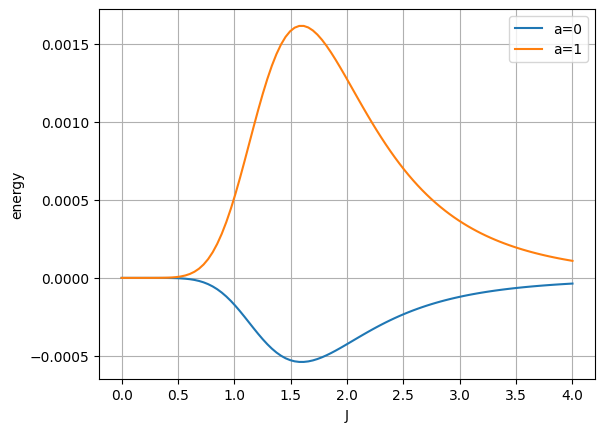
\includegraphics[width=\textwidth]{Appendix/plots/numerical/NearestNeighbors/Y_N4_energy_vs_J.png}
        \caption{\( \sigma_A = Y_0 \), \( N = 4 \)}
    \end{subfigure}

    \vspace{0.5em}

    \begin{subfigure}{0.33\textwidth}
        \centering
        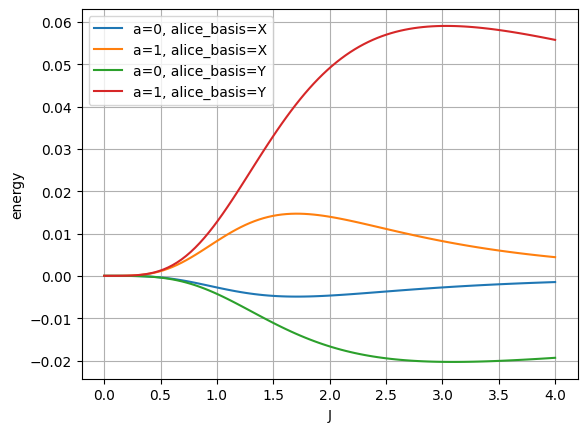
\includegraphics[width=\textwidth]{Appendix/plots/numerical/NearestNeighbors/both_N2_energy_vs_J.png}
        \caption{\( N = 2 \)}
    \end{subfigure}
    \hfill
    \begin{subfigure}{0.33\textwidth}
        \centering
        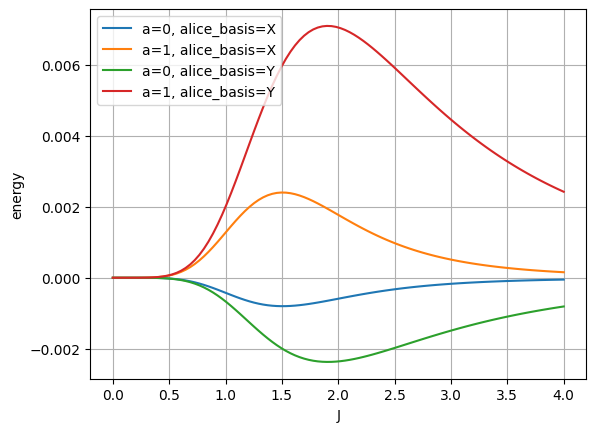
\includegraphics[width=\textwidth]{Appendix/plots/numerical/NearestNeighbors/both_N3_energy_vs_J.png}
        \caption{\( N = 3 \)}
    \end{subfigure}
    \hfill
    \begin{subfigure}{0.33\textwidth}
        \centering
        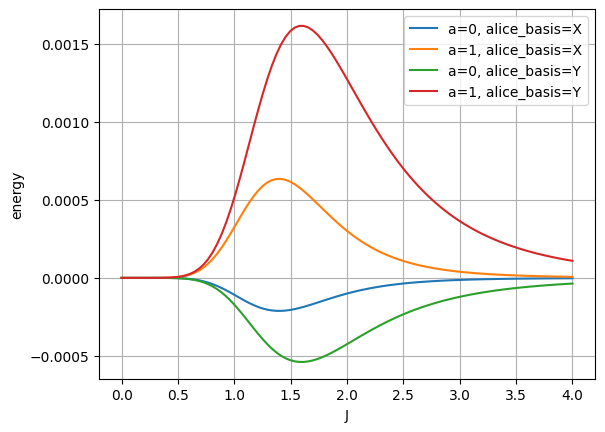
\includegraphics[width=\textwidth]{Appendix/plots/numerical/NearestNeighbors/both_N4_energy_vs_J.png}
        \caption{\( N = 4 \)}
    \end{subfigure}

    \caption{Extracted Energy value at Bob's site vs. \( J \), under nearest-neighbor Hamiltonian.}
    \label{fig:nn_vs_J}
\end{figure*}

\subsubsection{Summary of Observations}

\begin{itemize}
    \item The charge protocol remains strongly dependent on the basis choice, with the difference between X and Y observables increasing with \( N \).
    \item Energy teleportation results are more uniform across bases, indicating a \textbf{broader operational regime}.
    \item The field strength \( h \) controls the overall scale of extracted observables, but does not invert qualitative trends.
\end{itemize}

These findings reinforce the interpretation that energy teleportation offers \textbf{greater robustness to control imperfections}, while charge teleportation may provide \textbf{stronger signals} under optimized conditions.
